\section{The AVR MCU Series}
\label{sec:atmega_overview}

	In this paper we will focus on the ATmega644 board, of the Atmel AVR line of MCUs, as it is a widely available and popular low-cost microcontroller \citep{glitches_paper} . The AVR series is an enhanced-RISC architecture 8-bit MCU family that consists of the ATtiny, ATmega and ATxmega sub-categories,  32-bit AVRs and application specific FPGAs\cite{book:practical_avr}. The models have varying degrees of hardware capabilities and large operating voltage windows in order to accommodate demand and integrate well with peripherals\footnote{info:\href{https://www.newbiehack.com/MicrocontrollersAlternativePowerSources.aspx}{https://www.newbiehack.com}}\footnote{info:\href{http://www.atmel.com/v2PFResults.aspx}{http://www.atmel.com/v2PFResults.aspx}}. Developing software for an AVR is easy as the AVRs benefit from the  \texttt{avr-libc} high-performance library, the \texttt{avr-gcc} and \texttt{avr-gdb} compiler and debugger(both based on very popular and high quality GNU software tools), the \texttt{avrdude} programming software(or Atmel's \texttt{AVRStudio}) and \texttt{Simulavr} simulator software. Additionally, Atmel provides proprietary APIs for interacting with the AVR and the developers can choose from a wide variety of programmer units available for working with the AVRs\cite{book:practical_avr}.
	
	\subsection{ATMega Architecture and Features}				

	This paper will focus on the ATmega644, an enhanced-RISC Harvard architecture 8-bit CPU with a two stage pipeline and a total of 131 instructions. Fig.~\ref{fig:architectures} shows the conceptual difference between a Von Neuman and strict Harvard architecture, where the key distinction lies in the separation of application code and program data into different memory sections (Harvard) and tasking the CPU with distinguishing between code and data present in the same memory region (Von Neuman). The 644 implements a modified Harvard architecture for both power and computational efficiency, designed to access multiple memory locations simultaneously thus being able to execute an instruction per cycle, as shown in Fig.~\ref{fig:pipeline}. Their speed grades are  0-10~MHz for 2.7~V - 5.5~V and 0-20~MHz for 4.5~V - 5.5~V \citep{atmega_manual}.

	The 644 is equipped with 2 Kb of EEPROM, 64 Kb of flash memory, 4 Kb of SRAM, and a large number of general purpose (GP) and I/O registers and all memory (including memory mapped I/O images) is linear, i.e. it follows the flat memory model. The flash memory is separated into the bootloader and application code section and the boundary between the two sections, as well as the page size, can be configured by programming the appropriate fuses. Both sections hold code, however code residing in the bootloader section can execute the \texttt{SPM}\footnote{\texttt{SPM} = Store Program Code, assembly instruction for the AVR.} instruction which allows the bootloader code to write to \textit{any} section in the flash memory and hence possibly modify itself, facilitating purposes like firmware upgrades. The bootloader code can be triggered by a direct jump from the application section or by programming the reset vector via the reset fuse to point to the appropriate section of the bootloader code. The EEPROM is memory for data that needs to persist between reboots of the MCU and hence it is (widely) used to hold configuration variables and other non-temporary data the application code (or the bootloader) may need, having an average lifespan of 100,000 write cycles per page. The SRAM is volatile storage and is used as the stack and heap for the firmware and for storing the Register File, i.e. the 32 GP registers, I/O and Extended I/O Memory. The reserved register locations exist in order to support the use of peripheral units as well as hold program status information (e.g. the Stack Pointer can be found in one of the GP registers). Fig.~\ref{fig:stack} gives an overview of the SRAM hierarchy for the ATmega644.
	
	\begin{figure}
		\center
		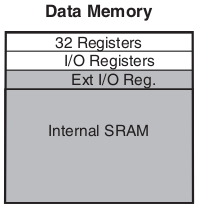
\includegraphics[scale=0.7]{img/stack.png}
		\caption{\footnotesize SRAM layout for ATmega644 (source: \protect\citep{atmega_manual}).}
		\label{fig:stack}		
	\end{figure}

	\begin{figure}
		\center
		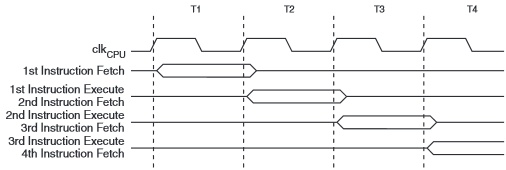
\includegraphics[scale=0.7]{img/pipeline.png}
		\caption{\footnotesize 2-stage pipeline of the ATmega644 (source: \protect\citep{atmega_manual}).}
		\label{fig:pipeline}		
	\end{figure}
	
\begin{figure*}
	\begin{subfigure}{0.5\textwidth}
		\center
		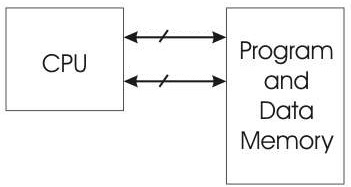
\includegraphics[scale=0.5]{img/von_neuman_arch.jpg}
		\caption{\footnotesize Typical Von Neuman architecture.}
		\label{fig:VN_arch}
	\end{subfigure} 
	~
	\begin{subfigure}{0.5\textwidth}
		\center
		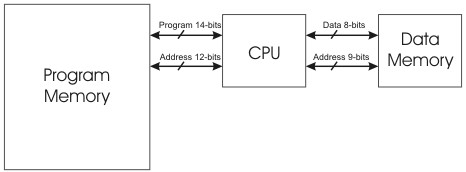
\includegraphics[scale=0.5]{img/harvard_arch.jpeg}
		\caption{\footnotesize Strict Harvard architecture.}
		\label{fig:H_arch}
	\end{subfigure}
	\caption{\footnotesize A comparison of different machine architectures (source: \protect\citep{website:mcu_primer}).}
	\label{fig:architectures}
\end{figure*}	
	
	\subsection{ATMega Security Features}
	
	The AVR ATmega644 is not meant to be a secure hardware module but offers firmware access control by using six lock bits responsible for controlling access to the board's memory and prevent reading or modifying the memory (e.g. prevent code executing from the bootloader section to read/write the application code section using \texttt{SPM}). This access control is not permanent, as that would limit the usefulness of the MCU and therefore one has the option to reset the lock bits (i.e. having no protection scheme enabled) by issuing a Chip Erase command, which has the effect of completely erasing the Flash, EEPROM and then the lock bits \citep{atmega_manual}. Chip erasing is performed with the sequence of events as presented and this is important, as one does not want to remove the access protection before removing all data and hence the lock bits are set to 1 only after the whole program memory has been erased. Even though the flash memory has an average lifespan of 10,000 write cycles, as well as programming being a relatively lengthy operation, this approach tries to preserve the intellectual property on the board rather than the board itself.
	
	\begin{table}
		\caption{\footnotesize Security lock bits offered by the ATmega644. BLB stands for Boot Lock Bit and LB for Lock Bit. (source: \protect\citep{tech:avrfreaks} \citep{atmega_manual})}
		\label{table:lock_bits}
		\center
		\begin{tabular}{| c | c | c | c |}
			\hline
			\textbf{Lock Bit Byte} & \textbf{Bit Number} & \textbf{Default}\\
			\hline \hline
			BLB12 & 5 & 1\\
			BLB11 & 4 & 1\\
			BLB02 & 3 & 1\\
			BLB01 & 2 & 1\\
			LB2 & 2 & 1 \\
			LB1 & 1 & 1 \\
			\hline
		\end{tabular}
		
	\end{table}
	
Table~\ref{table:lock_bits} presents an outline of the available Lock bits provided by the ATmega series. The functionality of the BLB1 group is to control access and modification of the bootloader section, group BLB0 bits control access to the application code section and group LB bits are responsible for controlling modifications on the EEPROM and Flash. A detailed explanation of their functionality and how to use them is given in the manuals \citep{atmega_manual} \citep{tech:avrfreaks}.
	